\documentclass{article}

% content/resources/templates/preamble.tex
\usepackage[margin=0.6in]{geometry}
\author{Milav Dabgar}
\usepackage{amsmath,amssymb,amsthm}
\usepackage{booktabs}
\usepackage{multirow}
\usepackage{xcolor}
\usepackage{tcolorbox}
\tcbuselibrary{breakable,skins}
\usepackage[colorlinks=true,linkcolor=blue]{hyperref}
\usepackage{titlesec}
\usepackage{enumitem}
\usepackage{tikz}
\usepackage{pgfplots}
\usepackage{circuitikz}
\usepackage[version=4]{mhchem}
\usepackage{longtable}
\usepackage{array}
\usepackage{float}
\usepackage{caption}
\usepackage{listings}

\lstset{
  basicstyle=\small\ttfamily,
  breaklines=true,
  breakatwhitespace=false,
  postbreak=\mbox{\textcolor{red}{$\hookrightarrow$}\space},
  float=false,
  numbers=left,
  numberstyle=\tiny\color{gray},
  numbersep=10pt,
  xleftmargin=2em,
  keywordstyle=\color{blue},
  commentstyle=\color{green!60!black},
  stringstyle=\color{purple},
  backgroundcolor=\color{gray!5},
  showstringspaces=false,
  tabsize=2,
  captionpos=b,
  keepspaces=true,
  columns=flexible
}

\pgfplotsset{compat=1.18}
\usetikzlibrary{shapes,arrows,positioning,calc,patterns,decorations.pathmorphing,decorations.markings,arrows.meta}

% Color scheme
\definecolor{headcolor}{RGB}{0,102,204}
\definecolor{keycolor}{RGB}{220,20,60}
\definecolor{solutioncolor}{RGB}{34,139,34}
\definecolor{mnemoniccolor}{RGB}{148,0,211}
\definecolor{codecolor}{RGB}{0,0,100}

% Spacing
\setlength{\parskip}{3pt}
\setlist[itemize]{nosep}
\setlist[enumerate]{nosep}

% Title formatting
\titleformat{\section}{\Large\bfseries\color{headcolor}}{\thesection}{1em}{}
\titleformat{\subsection}{\large\bfseries\color{headcolor}}{\thesubsection}{1em}{}

% Pandoc tightlist compatibility
\providecommand{\tightlist}{%
  \setlength{\itemsep}{0pt}\setlength{\parskip}{0pt}}

% Pandoc longtable compatibility
\newcounter{none}
\def\thenone{}


% content/resources/templates/english-boxes.tex

% Custom environments
\newtcolorbox{solutionbox}{
 breakable,
 enhanced,
 colback=solutioncolor!5!white,
 colframe=solutioncolor!75!black,
 fonttitle=\bfseries,
 title=Solution
}

\newtcolorbox{solutionboxnobreak}{
 colback=solutioncolor!5!white,
 colframe=solutioncolor!75!black,
 fonttitle=\bfseries,
 title=Solution
}

\newtcolorbox{keyformula}{
 breakable,
 enhanced,
 colback=keycolor!5!white,
 colframe=keycolor!75!black,
 fonttitle=\bfseries,
 title=Key Formula
}

\newtcolorbox{mnemonicboxenv}{
 breakable,
 enhanced,
 colback=mnemoniccolor!5!white,
 colframe=mnemoniccolor!75!black,
 fonttitle=\bfseries,
 title=Mnemonic
}

\newcommand{\mnemonicbox}[1]{%
  \begin{mnemonicboxenv}
    #1
  \end{mnemonicboxenv}
}


% Custom commands for GTU solutions
% This file defines semantic commands for consistent formatting

% Question command with automatic formatting
\newcommand{\question}[2]{%
  \section*{Question #1}%
  \textbf{#2}%
}

% OR question variant
\newcommand{\questionor}[2]{%
  \section*{Question #1 OR}%
  \textbf{#2}%
}

% Proper table environment with caption
\newenvironment{answertable}[1]{%
  \begin{table}[htbp]
  \centering
  \caption{#1}
}{%
  \end{table}
}

% Proper figure environment for diagrams
\newenvironment{answerdiagram}[1]{%
  \begin{figure}[htbp]
  \centering
  \caption{#1}
}{%
  \end{figure}
}

% Semantic markup for key terms
\newcommand{\keyword}[1]{\textbf{#1}}
\newcommand{\code}[1]{\texttt{#1}}
\newcommand{\classname}[1]{\texttt{#1}}
\newcommand{\methodname}[1]{\texttt{#1}}

% Proper quotation marks
\newcommand{\mnemonic}[1]{``#1''}


\title{Consumer Electronics and Maintenance (4341107) - Summer 2023 Solution}
\date{July 24, 2023}

\begin{document}
\maketitle

\questionmarks{1(a)}{3}{Describe maintenance procedure of CCTV.}
\begin{solutionbox}
    \begin{longtable}{|c|l|l|}
        \caption{CCTV Maintenance Procedure} \\
        \hline
        \textbf{Step} & \textbf{Procedure} & \textbf{Details} \\
        \hline
        1 & \textbf{Camera Cleaning} & Clean lenses and housings monthly \\
        \hline
        2 & \textbf{Cable Inspection} & Check for damage/exposure quarterly \\
        \hline
        3 & \textbf{Recording Check} & Verify data storage and playback monthly \\
        \hline
        4 & \textbf{Firmware Updates} & Update software when available \\
        \hline
        5 & \textbf{Angle Adjustment} & Realign cameras as needed \\
        \hline
    \end{longtable}

    \begin{mnemonicbox}
        \mnemonic{CCRU: Clean, Check, Record, Update}
    \end{mnemonicbox}
\end{solutionbox}

\questionmarks{1(b)}{4}{List the types of maintenance and explain in brief.}
\begin{solutionbox}
    \textbf{Table: Types of Maintenance} \\
\begin{tabulary}{\linewidth}{|l|L|L|L|}
        \hline
        \textbf{Type} & \textbf{Description} & \textbf{When Performed} & \textbf{Benefits} \\
        \hline
        \textbf{Preventive} & Regular checks before failure & Scheduled intervals & Reduces unexpected downtime \\
        \hline
        \textbf{Corrective} & Repairs after equipment breaks & After failure occurs & Restores functionality \\
        \hline
        \textbf{Predictive} & Uses data to predict failures & Based on analysis & Optimizes maintenance timing \\
        \hline
        \textbf{Condition-based} & Monitors actual equipment state & When conditions indicate & Reduces unnecessary maintenance \\
        \hline
    \end{tabulary}

    \begin{figure}[H]
        \centering
        \begin{tikzpicture}[gtu flow]
            \node (A) [gtu block] {Maintenance Types};
            \node (B) [gtu block, below left=1cm and 1cm of A] {Preventive};
            \node (C) [gtu block, below right=1cm and 1cm of A] {Corrective};
            \node (D) [gtu block, below left=3cm and 0.5cm of A] {Predictive};
            \node (E) [gtu block, below right=3cm and 0.5cm of A] {Condition-based};
            
            \draw [gtu arrow] (A) -- (B);
            \draw [gtu arrow] (A) -- (C);
            \draw [gtu arrow] (A) -- (D);
            \draw [gtu arrow] (A) -- (E);

            \node (F) [below=0.2cm of B, align=center, font=\footnotesize] {Scheduled checks};
            \node (G) [below=0.2cm of C, align=center, font=\footnotesize] {Repairs after breakdown};
            \node (H) [below=0.2cm of D, align=center, font=\footnotesize] {Data-based forecasting};
            \node (I) [below=0.2cm of E, align=center, font=\footnotesize] {Based on equipment condition};
        \end{tikzpicture}
        \caption{Types of Maintenance}
    \end{figure}

    \begin{mnemonicbox}
        \mnemonic{PCPC: Prevent, Correct, Predict, Condition}
    \end{mnemonicbox}
\end{solutionbox}

\questionmarks{1(c)}{7}{Explain maintenance and troubleshooting procedure of Washing Machine.}
\begin{solutionbox}
    \textbf{Table: Washing Machine Maintenance and Troubleshooting} \\
\begin{tabulary}{\linewidth}{|L|L|L|}
        \hline
        \textbf{Problem} & \textbf{Possible Cause} & \textbf{Troubleshooting Steps} \\
        \hline
        \textbf{Machine not starting} & Power issue, door lock & Check power supply, ensure door is closed properly \\
        \hline
        \textbf{Not filling with water} & Water supply, inlet valve & Check water taps, inspect inlet hoses for blocks \\
        \hline
        \textbf{Not draining} & Clogged filter, drain pump & Clean filter, check drain hose for kinks \\
        \hline
        \textbf{Excessive vibration} & Unbalanced load, shipping bolts & Redistribute clothes, check if shipping bolts removed \\
        \hline
        \textbf{Leaking water} & Damaged hoses, loose connections & Inspect and tighten connections, replace damaged hoses \\
        \hline
    \end{tabulary}

    \textbf{Regular Maintenance:}
    \begin{itemize}
        \item \textbf{Monthly}: Clean detergent drawer and door seal
        \item \textbf{Quarterly}: Run empty hot cycle with vinegar/cleaner
        \item \textbf{Bi-annually}: Check hoses for cracks, clean filter
    \end{itemize}

    \begin{figure}[H]
        \centering
        \begin{tikzpicture}[gtu flow]
            \node (A) [gtu block] {Problem Detected};
            \node (B) [gtu state, right=of A] {Machine Starts?};
            
            \node (C) [gtu block, below=of B] {Check Power \& Door Lock};
            \node (D) [gtu state, right=of B] {Fills with Water?};
            
            \node (E) [gtu block, below=of D] {Check Water Supply \& Inlet Valve};
            \node (F) [gtu state, right=of D] {Drains Properly?};
            
            \node (G) [gtu block, below=of F] {Check Filter \& Drain Pump};
            \node (H) [gtu state, right=of F] {Excessive Vibration?};
            
            \node (I) [gtu block, below=of H] {Check Load Balance \& Shipping Bolts};
            \node (J) [gtu state, right=of H] {Water Leakage?};
            
            \node (K) [gtu block, below=of J] {Check Hoses \& Connections};

            \draw [gtu arrow] (A) -- (B);
            \draw [gtu arrow] (B) -- node[left] {No} (C);
            \draw [gtu arrow] (B) -- node[above] {Yes} (D);
            
            \draw [gtu arrow] (D) -- node[left] {No} (E);
            \draw [gtu arrow] (D) -- node[above] {Yes} (F);
            
            \draw [gtu arrow] (F) -- node[left] {No} (G);
            \draw [gtu arrow] (F) -- node[above] {Yes} (H);
            
            \draw [gtu arrow] (H) -- node[left] {Yes} (I);
            \draw [gtu arrow] (H) -- node[above] {No} (J);
            
            \draw [gtu arrow] (J) -- node[left] {Yes} (K);
        \end{tikzpicture}
        \caption{Washing Machine Troubleshooting}
    \end{figure}

    \begin{mnemonicbox}
        \mnemonic{POWER: Power, Observe, Water, Examine, Repair}
    \end{mnemonicbox}
\end{solutionbox}

\questionmarks{1(c) OR}{7}{Explain maintenance and troubleshooting procedure of Digital TV.}
\begin{solutionbox}
    \textbf{Table: Digital TV Maintenance and Troubleshooting} \\
\begin{tabulary}{\linewidth}{|L|L|L|}
        \hline
        \textbf{Problem} & \textbf{Possible Cause} & \textbf{Troubleshooting Steps} \\
        \hline
        \textbf{No power} & Power supply issue & Check power cord, wall outlet, try different socket \\
        \hline
        \textbf{No picture} & Input/source selection & Verify correct input selected, check source device \\
        \hline
        \textbf{Poor reception} & Antenna/cable issue & Check cable connections, reposition antenna \\
        \hline
        \textbf{Distorted colors} & Display settings & Reset picture settings to default \\
        \hline
        \textbf{Remote not working} & Battery issue, sensor blocked & Replace batteries, ensure IR sensor not blocked \\
        \hline
    \end{tabulary}

    \textbf{Regular Maintenance:}
    \begin{itemize}
        \item \textbf{Weekly}: Dust screen carefully with microfiber cloth
        \item \textbf{Monthly}: Check and tighten cable connections
        \item \textbf{Annually}: Update firmware if available
    \end{itemize}

    \begin{figure}[H]
        \centering
        \begin{tikzpicture}[gtu flow]
            \node (A) [gtu block] {TV Problem};
            \node (B) [gtu state, right=of A] {Powers On?};
            \node (C) [gtu block, below=of B] {Check Power Supply};
            
            \node (D) [gtu state, right=of B] {Picture Visible?};
            \node (E) [gtu block, below=of D] {Check Input Source};
            
            \node (F) [gtu state, right=of D] {Good Reception?};
            \node (G) [gtu block, below=of F] {Check Antenna/Cable};
            
            \node (H) [gtu state, right=of F] {Correct Colors?};
            \node (I) [gtu block, below=of H] {Reset Picture Settings};
            
            \node (J) [gtu state, right=of H] {Remote Working?};
            \node (K) [gtu block, below=of J] {Check Batteries/Sensor};

            \draw [gtu arrow] (A) -- (B);
            \draw [gtu arrow] (B) -- node[right] {No} (C);
            \draw [gtu arrow] (B) -- node[above] {Yes} (D);
            
            \draw [gtu arrow] (D) -- node[right] {No} (E);
            \draw [gtu arrow] (D) -- node[above] {Yes} (F);
            
            \draw [gtu arrow] (F) -- node[right] {No} (G);
            \draw [gtu arrow] (F) -- node[above] {Yes} (H);
            
            \draw [gtu arrow] (H) -- node[right] {No} (I);
            \draw [gtu arrow] (H) -- node[above] {Yes} (J);
            
            \draw [gtu arrow] (J) -- node[right] {No} (K);
        \end{tikzpicture}
        \caption{TV Troubleshooting Flowchart}
    \end{figure}

    \begin{mnemonicbox}
        \mnemonic{SPIRE: Supply, Picture, Input, Reception, Electronics}
    \end{mnemonicbox}
\end{solutionbox}

\questionmarks{2(a)}{3}{Define: (1) Brightness (2) Luminance (3) Chrominance}
\begin{solutionbox}
    \textbf{Table: Key TV Display Terms} \\
\begin{tabulary}{\linewidth}{|l|L|L|}
        \hline
        \textbf{Term} & \textbf{Definition} & \textbf{Measured In} \\
        \hline
        \textbf{Brightness} & Perceived intensity of light output from display & Subjective perception (nits) \\
        \hline
        \textbf{Luminance} & Objective measurement of light intensity per unit area & Candela per square meter (cd/m$^2$) \\
        \hline
        \textbf{Chrominance} & Color information in video signal independent of brightness & U and V components \\
        \hline
    \end{tabulary}

    \begin{mnemonicbox}
        \mnemonic{BLC: Brightness is Light perception, Luminance is Calculated light, Chrominance is Color information}
    \end{mnemonicbox}
\end{solutionbox}

\questionmarks{2(b)}{4}{Draw and explain block diagram of DTH receiver.}
\begin{solutionbox}
    \textbf{DTH Receiver Block Diagram:}
    
    \begin{figure}[H]
        \centering
        \begin{tikzpicture}[gtu flow]
            \node (A) [gtu block] {Satellite Dish};
            \node (B) [gtu block, right=of A] {LNB};
            \node (C) [gtu block, right=of B] {Tuner};
            \node (D) [gtu block, below=of C] {Demodulator};
            \node (E) [gtu block, left=of D] {MPEG Decoder};
            
            \node (F) [gtu block, left=of E] {Video Processor};
            \node (G) [gtu block, below=of E] {Audio Processor};
            
            \node (H) [gtu block, left=of F] {TV Display};
            \node (I) [gtu block, left=of G] {Speakers};
            
            \node (J) [gtu block, below=of D] {Smart Card};
            \node (K) [gtu block, below=of J] {CAM};
            
            \node (L) [gtu block, right=of C] {User Interface};
            \node (M) [gtu block, below=of L] {Microcontroller};

            \draw [gtu arrow] (A) -- (B);
            \draw [gtu arrow] (B) -- (C);
            \draw [gtu arrow] (C) -- (D);
            \draw [gtu arrow] (D) -- (E);
            
            \draw [gtu arrow] (E) -- (F);
            \draw [gtu arrow] (E) -- (G);
            \draw [gtu arrow] (F) -- (H);
            \draw [gtu arrow] (G) -- (I);
            
            \draw [gtu arrow] (J) -- (K);
            \draw [gtu arrow] (K) -| (D);
            
            \draw [gtu arrow] (L) -- (M);
            \draw [gtu arrow] (M) -- (C);
            \draw [gtu arrow] (M) |- (E);
        \end{tikzpicture}
        \caption{DTH Receiver}
    \end{figure}

    \textbf{Table: DTH Receiver Components} \\
\begin{tabulary}{\linewidth}{|L|L|}
        \hline
        \textbf{Component} & \textbf{Function} \\
        \hline
        \textbf{Satellite Dish} & Receives satellite signals from space \\
        \hline
        \textbf{LNB (Low Noise Block)} & Converts high-frequency signals to lower frequency \\
        \hline
        \textbf{Tuner} & Selects specific channel frequency \\
        \hline
        \textbf{Demodulator} & Extracts digital data from carrier signal \\
        \hline
        \textbf{MPEG Decoder} & Decompresses audio/video data \\
        \hline
        \textbf{Conditional Access Module} & Controls subscription access \\
        \hline
    \end{tabulary}

    \begin{mnemonicbox}
        \mnemonic{SLTDM: Satellite captures, LNB converts, Tuner selects, Demodulator extracts, MPEG decodes}
    \end{mnemonicbox}
\end{solutionbox}

\questionmarks{2(c)}{7}{Draw and explain block diagram of colour TV receiver.}
\begin{solutionbox}
    \textbf{Colour TV Receiver Block Diagram:}

    \begin{figure}[H]
        \centering
        \begin{tikzpicture}[gtu flow]
            \node (A) [gtu block] {Antenna};
            \node (B) [gtu block, right=of A] {Tuner};
            \node (C) [gtu block, right=of B] {IF Amplifier};
            \node (D) [gtu block, right=of C] {Video Detector};
            
            \node (E) [gtu block, below=of D] {Video Amplifier};
            \node (F) [gtu block, right=of D] {Sound IF \& Detector};
            
            \node (G) [gtu block, left=of E] {Y Signal Processing};
            \node (H) [gtu block, below=of E] {Chrominance Bandpass};
            \node (I) [gtu block, below=of H] {Chroma Demodulator};
            
            \node (J) [gtu block, left=of I] {R-Y Signal};
            \node (K) [gtu block, below=of I] {B-Y Signal};
            
            \node (L) [gtu block, left=of G, text width=2.5cm] {RGB Matrix};
            \node (M) [gtu block, left=of L] {Picture Tube};
            
            \node (N) [gtu block, right=of F] {Audio Amplifier};
            \node (O) [gtu block, right=of N] {Speaker};
            \node (P) [gtu block, right=of B] {Power Supply};

            \draw [gtu arrow] (A) -- (B);
            \draw [gtu arrow] (B) -- (C);
            \draw [gtu arrow] (C) -- (D);
            \draw [gtu arrow] (D) -- (E);
            \draw [gtu arrow] (D) -- (F);
            
            \draw [gtu arrow] (E) -- (G);
            \draw [gtu arrow] (E) -- (H);
            \draw [gtu arrow] (H) -- (I);
            
            \draw [gtu arrow] (I) -- (J);
            \draw [gtu arrow] (I) -- (K);
            
            \draw [gtu arrow] (G) -- (L);
            \draw [gtu arrow] (J) -- (L);
            \draw [gtu arrow] (K) -| (L);
            
            \draw [gtu arrow] (L) -- (M);
            \draw [gtu arrow] (F) -- (N);
            \draw [gtu arrow] (N) -- (O);
            
            % Power supply lines (simplified)
            \draw [gtu arrow, dashed] (P) to[bend left] (C);
        \end{tikzpicture}
        \caption{Colour TV Receiver}
    \end{figure}

    \textbf{Table: Colour TV Components and Functions} \\
\begin{tabulary}{\linewidth}{|l|L|L|}
        \hline
        \textbf{Section} & \textbf{Function} & \textbf{Key Components} \\
        \hline
        \textbf{Tuner} & Selects desired channel & RF amplifier, mixer, local oscillator \\
        \hline
        \textbf{IF Amplifier} & Amplifies intermediate frequency & Bandpass filters, amplifiers \\
        \hline
        \textbf{Video Detector} & Extracts video signal & Diode detector, filters \\
        \hline
        \textbf{Chrominance Section} & Processes color information & Bandpass filter, color demodulator \\
        \hline
        \textbf{Luminance Section} & Processes brightness information & Y signal amplifier \\
        \hline
        \textbf{RGB Matrix} & Combines signals for display & Mixing circuits \\
        \hline
        \textbf{Audio Section} & Processes sound & Sound IF, detector, amplifier \\
        \hline
    \end{tabulary}

    \begin{mnemonicbox}
        \mnemonic{TIVACRL: Tuner tunes, IF amplifies, Video detects, Audio separates, Chrominance demodulates, RGB mixes, Light displays}
    \end{mnemonicbox}
\end{solutionbox}

\questionmarks{2(a) OR}{3}{Write a short note on LED TV.}
\begin{solutionbox}
    \textbf{Table: LED TV Technology} \\
\begin{tabulary}{\linewidth}{|l|L|}
        \hline
        \textbf{Aspect} & \textbf{Description} \\
        \hline
        \textbf{Basic Technology} & Uses Light Emitting Diodes for display backlighting \\
        \hline
        \textbf{Types} & Edge-lit (LEDs at edges), Direct-lit (LEDs behind screen), Full-array (with local dimming) \\
        \hline
        \textbf{Advantages} & Thinner profile, energy efficient, better contrast ratio, longer lifespan than LCD \\
        \hline
        \textbf{Display Panel} & Still uses LCD panel; LEDs are only for backlighting \\
        \hline
    \end{tabulary}

    \begin{mnemonicbox}
        \mnemonic{BEST: Backlighting with LEDs, Energy efficient, Slim design, True colors}
    \end{mnemonicbox}
\end{solutionbox}

\questionmarks{2(b) OR}{4}{Briefly explain the terms: (1) Hue (2) Saturation}
\begin{solutionbox}
    \textbf{Table: Color Properties} \\
\begin{tabulary}{\linewidth}{|l|L|L|L|}
        \hline
        \textbf{Term} & \textbf{Definition} & \textbf{Range} & \textbf{Example} \\
        \hline
        \textbf{Hue} & Actual color wavelength (red, blue, green, etc.) & 0-360 degrees on color wheel & Red=0$^\circ$, Green=120$^\circ$, Blue=240$^\circ$ \\
        \hline
        \textbf{Saturation} & Intensity or purity of color (how vivid) & 0-100\% (gray to pure color) & 0\%=grayscale, 100\%=vivid color \\
        \hline
    \end{tabulary}

    \begin{figure}[H]
        \centering
        \begin{tikzpicture}[gtu flow]
            \node (A) [gtu block] {Color Properties};
            \node (B) [gtu block, above right=of A] {Hue};
            \node (C) [gtu block, below right=of A] {Saturation};
            
            \node (D) [gtu block, right=of B] {Wavelength};
            \node (E) [gtu block, right=of C] {Purity};
            
            \node (F) [right=of D, font=\footnotesize] {0-360$^\circ$};
            \node (G) [right=of E, font=\footnotesize] {0-100\%};

            \draw [gtu arrow] (A) -- (B);
            \draw [gtu arrow] (A) -- (C);
            \draw [gtu arrow] (B) -- (D);
            \draw [gtu arrow] (C) -- (E);
            \draw [gtu arrow] (D) -- (F);
            \draw [gtu arrow] (E) -- (G);
        \end{tikzpicture}
        \caption{Color Hue and Saturation}
    \end{figure}

    \begin{mnemonicbox}
        \mnemonic{HS: Hue is the color Shade, Saturation is the color Strength}
    \end{mnemonicbox}
\end{solutionbox}

\questionmarks{2(c) OR}{7}{Explain additive colour mixing using colour circle diagram and Grassman's law.}
\begin{solutionbox}
    \textbf{Table: Additive Color Mixing Principles} \\
\begin{tabulary}{\linewidth}{|L|l|l|}
        \hline
        \textbf{Color Combination} & \textbf{Result} & \textbf{RGB Value} \\
        \hline
        \textbf{Red + Green} & Yellow & (255,255,0) \\
        \hline
        \textbf{Green + Blue} & Cyan & (0,255,255) \\
        \hline
        \textbf{Blue + Red} & Magenta & (255,0,255) \\
        \hline
        \textbf{Red + Green + Blue} & White & (255,255,255) \\
        \hline
        \textbf{No colors} & Black & (0,0,0) \\
        \hline
    \end{tabulary}

    \textbf{Grassman's Laws:}
    \begin{itemize}
        \item \textbf{Law 1}: Any color can be created by mixing three primary colors
        \item \textbf{Law 2}: The appearance of a color depends only on its tristimulus values
        \item \textbf{Law 3}: In additive mixing, the tristimulus values add together
    \end{itemize}

    \begin{figure}[H]
        \centering
        \begin{tikzpicture}[gtu flow]
            \node (P) [gtu block] {Primary Colors};
            \node (R) [gtu block, fill=red!20, below left=1.5cm and 2cm of P] {Red};
            \node (G) [gtu block, fill=green!20, below=1.5cm of P] {Green};
            \node (B) [gtu block, fill=blue!20, below right=1.5cm and 2cm of P] {Blue};
            
            \draw [gtu arrow] (P) -- (R);
            \draw [gtu arrow] (P) -- (G);
            \draw [gtu arrow] (P) -- (B);
            
            \node (Y) [gtu block, fill=yellow!20, below left=1.5cm of G] {Yellow};
            \node (C) [gtu block, fill=cyan!20, below right=1.5cm of G] {Cyan};
            \node (M) [gtu block, fill=magenta!20, below right=1.5cm and -1.5cm of Y] {Magenta};
            
            \draw [gtu arrow] (R) -- (Y);
            \draw [gtu arrow] (G) -- (Y);
            
            \draw [gtu arrow] (G) -- (C);
            \draw [gtu arrow] (B) -- (C);
            
            \draw [gtu arrow] (B) -- (M);
            \draw [gtu arrow] (R) -- (M);
            
            \node (W) [gtu block, fill=white, draw=black, below=2cm of G] {White};
            \draw [gtu arrow] (R) -- (W);
            \draw [gtu arrow] (G) -- (W);
            \draw [gtu arrow] (B) -- (W);
        \end{tikzpicture}
        \caption{Additive Mixing Flow}
    \end{figure}

    \textbf{Color Circle Diagram:}
    \begin{figure}[H]
        \centering
        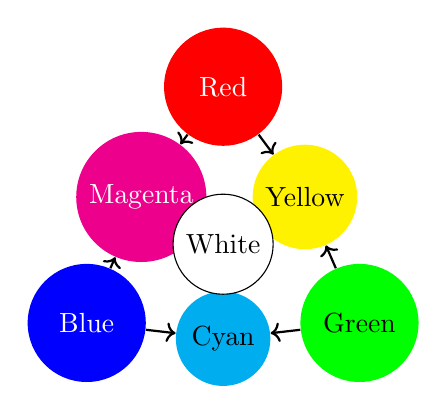
\begin{tikzpicture}
            \def\R{2}
            \coordinate (Center) at (0,0);
            
            \node (Red) at (90:\R) [circle, fill=red, text=white, minimum size=1.5cm] {Red};
            \node (Green) at (330:\R) [circle, fill=green, text=black, minimum size=1.5cm] {Green};
            \node (Blue) at (210:\R) [circle, fill=blue, text=white, minimum size=1.5cm] {Blue};
            
            \node (Yellow) at (30:{\R*0.6}) [circle, fill=yellow, text=black, minimum size=1.2cm] {Yellow};
            \node (Cyan) at (270:{\R*0.6}) [circle, fill=cyan, text=black, minimum size=1.2cm] {Cyan};
            \node (Magenta) at (150:{\R*0.6}) [circle, fill=magenta, text=white, minimum size=1.2cm] {Magenta};
            
            \node (White) at (0,0) [circle, fill=white, draw=black, minimum size=1cm] {White};
            
            \draw [thick, ->] (Red) -- (Yellow);
            \draw [thick, ->] (Green) -- (Yellow);
            
            \draw [thick, ->] (Green) -- (Cyan);
            \draw [thick, ->] (Blue) -- (Cyan);
            
            \draw [thick, ->] (Blue) -- (Magenta);
            \draw [thick, ->] (Red) -- (Magenta);
        \end{tikzpicture}
        \caption{Color Mixing Circle}
    \end{figure}

    \begin{mnemonicbox}
        \mnemonic{RGB-CMY-W: Red, Green, Blue make Cyan, Magenta, Yellow, and White}
    \end{mnemonicbox}
\end{solutionbox}

\questionmarks{3(a)}{3}{List wiring and safety instructions for microwave oven.}
\begin{solutionbox}
    \textbf{Table: Microwave Oven Wiring and Safety Instructions} \\
\begin{tabulary}{\linewidth}{|l|L|}
        \hline
        \textbf{Category} & \textbf{Instructions} \\
        \hline
        \textbf{Wiring} & Use grounded outlet with dedicated 15-20A circuit \\
        \hline
        \textbf{Power} & Ensure voltage matches rating (typically 220-240V) \\
        \hline
        \textbf{Installation} & Allow 5cm clearance on all sides for ventilation \\
        \hline
        \textbf{Safety} & Never operate empty, never bypass door interlocks \\
        \hline
        \textbf{Maintenance} & Disconnect power before servicing, discharge capacitor \\
        \hline
    \end{tabulary}

    \begin{mnemonicbox}
        \mnemonic{POWER: Proper Outlet, Wiring check, Empty operation avoided, Repairs by professionals}
    \end{mnemonicbox}
\end{solutionbox}

\questionmarks{3(b)}{4}{Explain working of Air conditioner.}
\begin{solutionbox}
    \textbf{Table: Air Conditioner Working Cycle} \\
\begin{tabulary}{\linewidth}{|l|L|L|}
        \hline
        \textbf{Component} & \textbf{Function} & \textbf{Process} \\
        \hline
        \textbf{Compressor} & Pressurizes refrigerant & Converts low-pressure gas to high-pressure gas \\
        \hline
        \textbf{Condenser} & Releases heat outside & Converts gas to liquid, expels heat \\
        \hline
        \textbf{Expansion Valve} & Regulates refrigerant flow & Reduces pressure of liquid \\
        \hline
        \textbf{Evaporator} & Absorbs heat from room & Converts liquid to gas, cools air \\
        \hline
        \textbf{Thermostat} & Controls temperature & Regulates compressor operation \\
        \hline
    \end{tabulary}

    \begin{figure}[H]
        \centering
        \begin{tikzpicture}[gtu flow]
            \node (Comp) [gtu block] {Compressor};
            \node (Cond) [gtu block, right=2cm of Comp] {Condenser};
            \node (Exp) [gtu block, below=2cm of Cond] {Expansion Valve};
            \node (Evap) [gtu block, below=2cm of Comp] {Evaporator};
            
            \draw [gtu arrow] (Comp) -- node[above, font=\footnotesize] {High-P Gas} (Cond);
            \draw [gtu arrow] (Cond) -- node[right, font=\footnotesize] {Liquid} (Exp);
            \draw [gtu arrow] (Exp) -- node[below, font=\footnotesize] {Low-P Liquid} (Evap);
            \draw [gtu arrow] (Evap) -- node[left, font=\footnotesize] {Low-P Gas} (Comp);
            
            \node (In) [left=of Evap, align=center] {Room Air};
            \node (Out) [right=of Evap, align=center] {Cool Air};
            \draw [gtu arrow] (In) -- (Evap);
            \draw [gtu arrow] (Evap) -- (Out);
            
            \node (Outside) [left=of Cond, align=center] {Outside Air};
            \node (Hot) [right=of Cond, align=center] {Hot Air};
            \draw [gtu arrow] (Outside) -- (Cond);
            \draw [gtu arrow] (Cond) -- (Hot);
        \end{tikzpicture}
        \caption{Air Conditioner Cycle}
    \end{figure}

    \begin{mnemonicbox}
        \mnemonic{CELT: Compress gas, Expel heat, Lower pressure, Take in heat}
    \end{mnemonicbox}
\end{solutionbox}

\questionmarks{3(c)}{7}{Explain electronic controller for washing machine and fuzzy logic washing machine. Also list technical specifications of washing machine.}
\begin{solutionbox}
    \textbf{Table: Electronic Controller in Washing Machines} \\
\begin{tabulary}{\linewidth}{|l|L|}
        \hline
        \textbf{Component} & \textbf{Function} \\
        \hline
        \textbf{Microcontroller} & Central processing unit controlling all operations \\
        \hline
        \textbf{Sensors} & Detect water level, temperature, load balance, door status \\
        \hline
        \textbf{Input Interface} & Buttons/touch panel for program selection \\
        \hline
        \textbf{Display} & Shows program status, time remaining, error codes \\
        \hline
        \textbf{Actuator Drivers} & Control motor, valves, heater, pump \\
        \hline
    \end{tabulary}

    \textbf{Fuzzy Logic in Washing Machines:}
    \begin{itemize}
        \item Uses artificial intelligence for optimal washing
        \item Adjusts water level, wash time, and spin speed based on load
        \item Makes decisions using approximate reasoning instead of precise values
        \item Adapts to different fabric types and soil levels automatically
    \end{itemize}

    \textbf{Technical Specifications:}
    \begin{itemize}
        \item \textbf{Capacity}: 6-10 kg (front load), 5-8 kg (top load)
        \item \textbf{Energy Rating}: A+++ to B (EU standards)
        \item \textbf{Water Consumption}: 40-70 liters per cycle
        \item \textbf{Spin Speed}: 800-1600 RPM
        \item \textbf{Cycle Options}: 8-16 programs
    \end{itemize}

    \begin{figure}[H]
        \centering
        \begin{tikzpicture}[gtu flow]
            \node (MC) [gtu block, minimum width=3cm, minimum height=2cm] {Electronic Controller\\(Microcontroller)};
            
            \node (Sens) [gtu block, left=2cm of MC] {Sensors};
            \node (UI) [gtu block, above=1cm of MC] {User Interface};
            \node (Fuzzy) [gtu block, below=1cm of MC] {Fuzzy Logic};
            \node (Act) [gtu block, right=2cm of MC] {Actuators};
            
            \draw [gtu arrow] (Sens) -- (MC);
            \draw [gtu arrow] (UI) -- (MC);
            \draw [gtu arrow] (Fuzzy) -- (MC);
            \draw [gtu arrow] (MC) -- (Act);
            
            % Detail inputs/outputs
            \node [left=0.2cm of Sens, align=right, font=\footnotesize] {Water Level\\Temp\\Load Balance\\Door Lock};
            \node [right=0.2cm of Act, align=left, font=\footnotesize] {Motor\\Water Valve\\Drain Pump\\Heater};
        \end{tikzpicture}
        \caption{Washing Machine Controller}
    \end{figure}

    \begin{mnemonicbox}
        \mnemonic{SCRAM: Sensors detect, Controller processes, Rules applied, Actuators operate, Machine adapts}
    \end{mnemonicbox}
\end{solutionbox}

\questionmarks{3(a) OR}{3}{State main components of solar power system and specifications of solar power system.}
\begin{solutionbox}
    \textbf{Table: Solar Power System Components} \\
\begin{tabulary}{\linewidth}{|l|L|}
        \hline
        \textbf{Component} & \textbf{Function} \\
        \hline
        \textbf{Solar Panels} & Convert sunlight to DC electricity \\
        \hline
        \textbf{Inverter} & Converts DC to AC power \\
        \hline
        \textbf{Battery Bank} & Stores energy for later use \\
        \hline
        \textbf{Charge Controller} & Prevents battery overcharging \\
        \hline
        \textbf{Mounting Structure} & Supports and angles panels optimally \\
        \hline
    \end{tabulary}

    \textbf{Specifications:}
    \begin{itemize}
        \item \textbf{Panel Capacity}: 250-400 Watts per panel
        \item \textbf{System Size}: 1-10 kW (residential)
        \item \textbf{Battery Capacity}: 100-200 Ah
        \item \textbf{Inverter Efficiency}: 90-97\%
        \item \textbf{Expected Lifespan}: 25-30 years (panels)
    \end{itemize}

    \begin{mnemonicbox}
        \mnemonic{PIBCM: Panels collect, Inverter converts, Batteries store, Controller protects, Mounts support}
    \end{mnemonicbox}
\end{solutionbox}

\questionmarks{3(b) OR}{4}{Explain working of Refrigerator.}
\begin{solutionbox}
    \textbf{Table: Refrigerator Working Cycle} \\
\begin{tabulary}{\linewidth}{|c|l|l|L|}
        \hline
        \textbf{Stage} & \textbf{Process} & \textbf{Component} & \textbf{State of Refrigerant} \\
        \hline
        1 & Compression & Compressor & Low pressure gas $\rightarrow$ High pressure gas \\
        \hline
        2 & Condensation & Condenser coils & High pressure gas $\rightarrow$ High pressure liquid \\
        \hline
        3 & Expansion & Expansion valve & High pressure liquid $\rightarrow$ Low pressure liquid \\
        \hline
        4 & Evaporation & Evaporator coils & Low pressure liquid $\rightarrow$ Low pressure gas \\
        \hline
    \end{tabulary}

    \begin{figure}[H]
        \centering
        \begin{tikzpicture}[gtu flow]
            \node (Comp) [gtu block] {Compressor};
            \node (Cond) [gtu block, right=2cm of Comp] {Condenser};
            \node (Exp) [gtu block, below=2cm of Cond] {Expansion Valve};
            \node (Evap) [gtu block, below=2cm of Comp] {Evaporator};
            
            \draw [gtu arrow] (Comp) -- node[above, font=\footnotesize] {High-P Gas} (Cond);
            \draw [gtu arrow] (Cond) -- node[right, font=\footnotesize] {High-P Liquid} (Exp);
            \draw [gtu arrow] (Exp) -- node[below, font=\footnotesize] {Low-P Liquid} (Evap);
            \draw [gtu arrow] (Evap) -- node[left, font=\footnotesize] {Low-P Gas} (Comp);
            
            \node (HeatOut) [above=0.5cm of Cond, font=\footnotesize] {Heat Released Outside};
            \draw [->, thick] (Cond) -- (HeatOut);
            
            \node (HeatIn) [below=0.5cm of Evap, font=\footnotesize] {Heat Absorbed Inside};
            \draw [->, thick] (HeatIn) -- (Evap);
            
            \node (Thermo) [left=of Comp, font=\footnotesize] {Thermostat};
            \draw [gtu arrow] (Thermo) -- (Comp);
        \end{tikzpicture}
        \caption{Refrigerator Cycle}
    \end{figure}

    \begin{mnemonicbox}
        \mnemonic{CEHE: Compress gas, Expel heat, Halve pressure, Extract heat}
    \end{mnemonicbox}
\end{solutionbox}

\questionmarks{3(c) OR}{7}{Draw and explain block diagram of Microwave oven. List types, applications and technical specifications of microwave oven.}
\begin{solutionbox}
    \textbf{Microwave Oven Block Diagram:}

    \begin{figure}[H]
        \centering
        \begin{tikzpicture}[gtu flow]
            \node (PS) [gtu block] {Power Supply};
            \node (Control) [gtu block, below=of PS] {Control Panel};
            \node (HV) [gtu block, right=of PS] {HV Transformer};
            \node (Circuit) [gtu block, below=of HV] {Control Circuit};
            
            \node (Magnetron) [gtu block, right=of HV] {Magnetron};
            \node (Wave) [gtu block, right=of Magnetron] {Waveguide};
            \node (Cavity) [gtu block, below=of Wave] {Cooking Cavity};
            
            \node (Motor) [gtu block, below=of Cavity] {Turntable Motor};
            
            \draw [gtu arrow] (PS) -- (HV);
            \draw [gtu arrow] (PS) -- (Control);
            \draw [gtu arrow] (Control) -- (Circuit);
            
            \draw [gtu arrow] (HV) -- (Magnetron);
            \draw [gtu arrow] (Magnetron) -- (Wave);
            \draw [gtu arrow] (Wave) -- (Cavity);
            
            \draw [gtu arrow] (Circuit) -| (Motor);
            \draw [gtu arrow] (Circuit) -- node[right, font=\footnotesize] {Controls} (HV);
        \end{tikzpicture}
        \caption{Microwave Oven Block Diagram}
    \end{figure}

    \textbf{Types of Microwave Ovens:}
    \begin{itemize}
        \item \textbf{Solo}: Basic heating and defrosting only
        \item \textbf{Grill}: Has additional grilling element
        \item \textbf{Convection}: Combines microwave with convection heating
        \item \textbf{Over-the-Range (OTR)}: Includes ventilation system
        \item \textbf{Built-in}: Designed for cabinet installation
    \end{itemize}

    \textbf{Applications:}
    \begin{itemize}
        \item \textbf{Cooking}: Fast meal preparation
        \item \textbf{Reheating}: Leftover foods
        \item \textbf{Defrosting}: Frozen foods
        \item \textbf{Sterilization}: Small items
        \item \textbf{Commercial}: Food service industry
    \end{itemize}

    \textbf{Technical Specifications:}
    \begin{itemize}
        \item \textbf{Capacity}: 20-40 liters
        \item \textbf{Power Output}: 700-1200 watts
        \item \textbf{Power Consumption}: 1100-1500 watts
        \item \textbf{Frequency}: 2.45 GHz
        \item \textbf{Voltage}: 220-240V AC
    \end{itemize}

    \begin{mnemonicbox}
        \mnemonic{MICROWAVES: Magnetron generates, Interior receives, Control regulates, Rotating turntable, Oven cavity, Waveguide directs, Alternating current powers, Ventilation cools, Electronic timer, Safety interlocks}
    \end{mnemonicbox}
\end{solutionbox}

\questionmarks{4(a)}{3}{List specifications of MF printer and LCD projector.}
\begin{solutionbox}
    \textbf{Table: Multi-Function Printer Specifications} \\
\begin{tabulary}{\linewidth}{|l|l|}
        \hline
        \textbf{Specification} & \textbf{Typical Range} \\
        \hline
        \textbf{Print Resolution} & 600-4800 dpi \\
        \hline
        \textbf{Print Speed} & 20-40 ppm (black), 15-30 ppm (color) \\
        \hline
        \textbf{Scan Resolution} & 600-1200 dpi \\
        \hline
        \textbf{Connectivity} & Wi-Fi, Ethernet, USB, Cloud \\
        \hline
        \textbf{Paper Capacity} & 100-500 sheets \\
        \hline
    \end{tabulary}

    \textbf{Table: LCD Projector Specifications} \\
\begin{tabulary}{\linewidth}{|l|l|}
        \hline
        \textbf{Specification} & \textbf{Typical Range} \\
        \hline
        \textbf{Brightness} & 2000-5000 lumens \\
        \hline
        \textbf{Resolution} & XGA (1024$\times$768) to 4K (3840$\times$2160) \\
        \hline
        \textbf{Contrast Ratio} & 2000:1 to 100,000:1 \\
        \hline
        \textbf{Lamp Life} & 4000-8000 hours \\
        \hline
        \textbf{Connectivity} & HDMI, VGA, USB, Wireless \\
        \hline
    \end{tabulary}

    \begin{mnemonicbox}
        \mnemonic{PSCPL: Print resolution, Speed, Connectivity, Projection brightness, Lamp life}
    \end{mnemonicbox}
\end{solutionbox}

\questionmarks{4(b)}{4}{Draw block diagram of Inkjet printer and explain its working in brief.}
\begin{solutionbox}
    \textbf{Inkjet Printer Block Diagram:}

    \begin{figure}[H]
        \centering
        \begin{tikzpicture}[gtu flow]
            \node (Control) [gtu block] {Control Board/CPU};
            \node (PS) [gtu block, left=of Control] {Power Supply};
            \node (Interface) [gtu block, right=of Control] {Interface};
            \node (PC) [gtu block, right=of Interface] {Computer};
            
            \node (PaperMotor) [gtu block, below left=1.5cm of Control] {Paper Feed Motor};
            \node (PrintMotor) [gtu block, below=1.5cm of Control] {Carriage Motor};
            \node (HeadControl) [gtu block, below right=1.5cm of Control] {Printhead Controller};
            
            \node (Mech) [gtu block, below=of PaperMotor] {Mechanism};
            \node (Carriage) [gtu block, below=of PrintMotor] {Carriage};
            \node (Cartridge) [gtu block, below=of HeadControl] {Ink Cartridges};
            \node (Nozzle) [gtu block, below=of Cartridge] {Nozzles};
            
            \draw [gtu arrow] (PS) -- (Control);
            \draw [gtu arrow] (PC) -- (Interface);
            \draw [gtu arrow] (Interface) -- (Control);
            
            \draw [gtu arrow] (Control) -- (PaperMotor);
            \draw [gtu arrow] (Control) -- (PrintMotor);
            \draw [gtu arrow] (Control) -- (HeadControl);
            
            \draw [gtu arrow] (PaperMotor) -- (Mech);
            \draw [gtu arrow] (PrintMotor) -- (Carriage);
            \draw [gtu arrow] (HeadControl) -- (Cartridge);
            \draw [gtu arrow] (Cartridge) -- (Nozzle);
            \draw [gtu arrow] (Carriage) -- (Cartridge);
        \end{tikzpicture}
        \caption{Inkjet Printer}
    \end{figure}

    \textbf{Working of Inkjet Printer:}
    \begin{enumerate}
        \item \textbf{Document Processing}: Control board receives data and converts to printer commands
        \item \textbf{Paper Loading}: Feed motor pulls paper from tray
        \item \textbf{Printing}: Printhead moves across paper while ejecting tiny ink droplets
        \item \textbf{Droplet Formation}: Thermal or piezoelectric method forces ink droplets onto paper
        \item \textbf{Paper Advancement}: Paper advances line by line until printing completes
    \end{enumerate}

    \begin{mnemonicbox}
        \mnemonic{PIPES: Paper feeds, Ink ejects, Printhead moves, Electronic control, Sheet advances}
    \end{mnemonicbox}
\end{solutionbox}

\questionmarks{4(c)}{7}{Explain working of Photocopier with block diagram and list its specifications.}
\begin{solutionbox}
    \textbf{Photocopier Block Diagram:}

    \begin{figure}[H]
        \centering
        \begin{tikzpicture}[gtu flow]
            \node (Main) [gtu block] {Main Control};
            \node (Scan) [gtu block, left=of Main] {Scanner/Optics};
            \node (Image) [gtu block, right=of Main] {Imaging System};
            \node (Paper) [gtu block, below=of Main] {Paper Feed};
            
            \node (Mirror) [gtu block, below=of Scan] {Mirrors/Lens};
            \node (Drum) [gtu block, below=of Image] {Photosensitive Drum};
            
            \node (Charge) [gtu block, right=of Drum] {Charging};
            \node (Dev) [gtu block, below=of Drum] {Developer};
            \node (Trans) [gtu block, left=of Drum] {Transfer};
            \node (Fuse) [gtu block, below=of Trans] {Fuser};
            
            \draw [gtu arrow] (Main) -- (Scan);
            \draw [gtu arrow] (Main) -- (Image);
            \draw [gtu arrow] (Main) -- (Paper);
            
            \draw [gtu arrow] (Scan) -- (Mirror);
            \draw [gtu arrow] (Mirror) -- (Drum);
            
            \draw [gtu arrow] (Charge) -- (Drum);
            \draw [gtu arrow] (Dev) -- (Drum);
            \draw [gtu arrow] (Drum) -- (Trans);
            \draw [gtu arrow] (Paper) -| (Trans);
            \draw [gtu arrow] (Trans) -- (Fuse);
        \end{tikzpicture}
        \caption{Photocopier System}
    \end{figure}

    \textbf{Working of Photocopier:}
    \begin{enumerate}
        \item \textbf{Charging}: Photosensitive drum receives uniform electrostatic charge
        \item \textbf{Exposure}: Original document scanned, creating light pattern on drum
        \item \textbf{Developing}: Toner particles attracted to charged areas on drum
        \item \textbf{Transfer}: Toner image transferred from drum to paper
        \item \textbf{Fusing}: Heat and pressure melt toner permanently onto paper
        \item \textbf{Cleaning}: Drum cleaned for next cycle
    \end{enumerate}

    \textbf{Technical Specifications:}
    \begin{itemize}
        \item \textbf{Speed}: 20-60 pages per minute
        \item \textbf{Resolution}: 600-1200 dpi
        \item \textbf{Paper Capacity}: 250-2000 sheets
        \item \textbf{Maximum Paper Size}: A3/11$\times$17 inches
        \item \textbf{Zoom Range}: 25-400\%
        \item \textbf{Memory}: 512MB-2GB
        \item \textbf{Connectivity}: Ethernet, USB, Wi-Fi
    \end{itemize}

    \begin{mnemonicbox}
        \mnemonic{CETFC: Charge drum, Expose image, Transfer toner, Fuse permanently, Clean drum}
    \end{mnemonicbox}
\end{solutionbox}

\questionmarks{4(a) OR}{3}{Write a short note on CCTV.}
\begin{solutionbox}
    \textbf{Table: CCTV System Overview} \\
\begin{tabulary}{\linewidth}{|l|L|}
        \hline
        \textbf{Aspect} & \textbf{Description} \\
        \hline
        \textbf{Full Form} & Closed-Circuit Television \\
        \hline
        \textbf{Purpose} & Security monitoring and surveillance \\
        \hline
        \textbf{Components} & Cameras, DVR/NVR, monitors, cables, power supply \\
        \hline
        \textbf{Types} & Analog, IP (digital), Wireless, HD-CVI/TVI/SDI \\
        \hline
        \textbf{Features} & Motion detection, night vision, remote viewing \\
        \hline
    \end{tabulary}

    \textbf{Key Applications:}
    \begin{itemize}
        \item Security monitoring of buildings
        \item Traffic monitoring
        \item Retail loss prevention
        \item Public area surveillance
        \item Home security
    \end{itemize}

    \begin{mnemonicbox}
        \mnemonic{SCRAM: Security monitoring, Closed circuit, Recording footage, Access restricted, Monitoring continuous}
    \end{mnemonicbox}
\end{solutionbox}

\questionmarks{4(b) OR}{4}{Explain working of LCD projector with block diagram.}
\begin{solutionbox}
    \textbf{LCD Projector Block Diagram:}

    \begin{figure}[H]
        \centering
        \begin{tikzpicture}[gtu flow]
            \node (Lamp) [gtu block] {Lamp};
            \node (Mirror) [gtu block, right=of Lamp] {Dichroic Mirrors};
            
            \node (R) [gtu block, right=of Mirror, fill=red!20] {Red LCD};
            \node (G) [gtu block, above=of Mirror, fill=green!20] {Green LCD};
            \node (B) [gtu block, below=of Mirror, fill=blue!20] {Blue LCD};
            
            \node (Prism) [gtu block, right=3cm of Mirror] {Prism};
            \node (Lens) [gtu block, right=of Prism] {Lens};
            \node (Screen) [gtu block, right=of Lens] {Screen};
            
            \draw [gtu arrow] (Lamp) -- (Mirror);
            \draw [gtu arrow] (Mirror) -- (R);
            \draw [gtu arrow] (Mirror) -- (G);
            \draw [gtu arrow] (Mirror) -- (B);
            
            \draw [gtu arrow] (R) -- (Prism);
            \draw [gtu arrow] (G) -- (Prism);
            \draw [gtu arrow] (B) -- (Prism);
            
            \draw [gtu arrow] (Prism) -- (Lens);
            \draw [gtu arrow] (Lens) -- (Screen);
            
            \node (Control) [gtu block, below=of Prism] {Control Circuit};
            \draw [gtu arrow] (Control) -- (R);
            \draw [gtu arrow] (Control) -- (G);
            \draw [gtu arrow] (Control) -- (B);
        \end{tikzpicture}
        \caption{LCD Projector}
    \end{figure}

    \textbf{Working of LCD Projector:}
    \begin{enumerate}
        \item \textbf{Light Generation}: High-intensity lamp produces white light
        \item \textbf{Color Separation}: Dichroic mirrors split light into RGB components
        \item \textbf{Image Formation}: LCD panels modulate light based on input signal
        \item \textbf{Recombination}: Prism combines RGB images into full-color image
        \item \textbf{Projection}: Lens system projects final image onto screen
    \end{enumerate}

    \begin{mnemonicbox}
        \mnemonic{LSCIP: Light source generates, Split into colors, Control with LCDs, Image combined, Projected on screen}
    \end{mnemonicbox}
\end{solutionbox}

\questionmarks{4(c) OR}{7}{Explain working of laser printer with block diagram.}
\begin{solutionbox}
    \textbf{Laser Printer Block Diagram:}

    \begin{figure}[H]
        \centering
        \begin{tikzpicture}[gtu flow]
            \node (Control) [gtu block] {Control Board};
            
            \node (Laser) [gtu block, right=of Control] {Laser Diode};
            \node (Mirror) [gtu block, right=of Laser] {Polygon Mirror};
            \node (Drum) [gtu block, below=of Mirror] {Photosensitive Drum};
            
            \node (Charge) [gtu block, right=of Drum] {Charging};
            \node (Dev) [gtu block, below=of Drum] {Developer};
            \node (Trans) [gtu block, left=of Drum] {Transfer};
            \node (Fuse) [gtu block, below=of Trans] {Fuser};
            
            \draw [gtu arrow] (Control) -- (Laser);
            \draw [gtu arrow] (Laser) -- (Mirror);
            \draw [gtu arrow] (Mirror) -- (Drum);
            
            \draw [gtu arrow] (Charge) -- (Drum);
            \draw [gtu arrow] (Dev) -- (Drum);
            \draw [gtu arrow] (Drum) -- (Trans);
            \draw [gtu arrow] (Trans) -- (Fuse);
            
            \node (Paper) [gtu block, left=of Trans] {Paper Path};
            \draw [gtu arrow] (Paper) -- (Trans);
        \end{tikzpicture}
        \caption{Laser Printer}
    \end{figure}

    \textbf{Laser Printing Process:}
    \textbf{Table: Six Steps of Laser Printing} \\
\begin{tabulary}{\linewidth}{|c|L|L|L|}
        \hline
        \textbf{Step} & \textbf{Process} & \textbf{Component} & \textbf{Function} \\
        \hline
        1 & \textbf{Cleaning} & Cleaning blade & Removes residual toner from drum \\
        \hline
        2 & \textbf{Charging} & Primary corona & Applies uniform negative charge to drum \\
        \hline
        3 & \textbf{Writing} & Laser \& mirror & Creates electrostatic image on drum \\
        \hline
        4 & \textbf{Developing} & Developer unit & Applies toner to charged areas of drum \\
        \hline
        5 & \textbf{Transferring} & Transfer corona & Moves toner from drum to paper \\
        \hline
        6 & \textbf{Fusing} & Fuser unit & Melts toner permanently onto paper \\
        \hline
    \end{tabulary}

    \textbf{Technical Specifications:}
    \begin{itemize}
        \item \textbf{Print Speed}: 20-50 ppm
        \item \textbf{Resolution}: 600-2400 dpi
        \item \textbf{Memory}: 128MB-1GB
        \item \textbf{Duty Cycle}: 10,000-150,000 pages/month
        \item \textbf{Connectivity}: USB, Ethernet, Wi-Fi
    \end{itemize}

    \begin{mnemonicbox}
        \mnemonic{CCWDTF: Clean drum, Charge uniformly, Write with laser, Develop with toner, Transfer to paper, Fuse permanently}
    \end{mnemonicbox}
\end{solutionbox}

\questionmarks{5(a)}{3}{Define: (1) Pitch (2) Reverberation (3) Microphone.}
\begin{solutionbox}
    \textbf{Table: Audio Terminology} \\
\begin{tabulary}{\linewidth}{|l|L|l|}
        \hline
        \textbf{Term} & \textbf{Definition} & \textbf{Measured In} \\
        \hline
        \textbf{Pitch} & Perceived frequency of sound; how high or low a tone seems & Hertz (Hz) \\
        \hline
        \textbf{Reverberation} & Persistence of sound after source stops; caused by reflections & Seconds (RT60) \\
        \hline
        \textbf{Microphone} & Transducer that converts sound waves into electrical signals & Sensitivity in dB/mV/Pa \\
        \hline
    \end{tabulary}

    \begin{mnemonicbox}
        \mnemonic{PRM: Pitch is frequency, Reverberation is reflection, Microphone is converter}
    \end{mnemonicbox}
\end{solutionbox}

\questionmarks{5(b)}{4}{Draw and explain block diagram of PA system.}
\begin{solutionbox}
    \textbf{PA System Block Diagram:}

    \begin{figure}[H]
        \centering
        \begin{tikzpicture}[gtu flow]
            \node (Mic) [gtu block] {Microphone};
            \node (Pre) [gtu block, right=of Mic] {Pre-amplifier};
            \node (Mixer) [gtu block, right=of Pre] {Mixer};
            \node (Source) [gtu block, above=of Mixer] {Audio Source};
            \node (EQ) [gtu block, right=of Mixer] {Equalizer};
            \node (Power) [gtu block, right=of EQ] {Power Amplifier};
            \node (Speaker) [gtu block, right=of Power] {Speaker System};
            \node (Control) [gtu block, below=of Mixer] {Control System};
            
            \draw [gtu arrow] (Mic) -- (Pre);
            \draw [gtu arrow] (Pre) -- (Mixer);
            \draw [gtu arrow] (Source) -- (Mixer);
            \draw [gtu arrow] (Mixer) -- (EQ);
            \draw [gtu arrow] (EQ) -- (Power);
            \draw [gtu arrow] (Power) -- (Speaker);
            \draw [gtu arrow] (Control) -| (Power);
            \draw [gtu arrow] (Control) -- (Mixer);
        \end{tikzpicture}
        \caption{Public Address System}
    \end{figure}

    \textbf{Table: PA System Components} \\
\begin{tabulary}{\linewidth}{|l|L|}
        \hline
        \textbf{Component} & \textbf{Function} \\
        \hline
        \textbf{Microphone} & Captures sound and converts to electrical signals \\
        \hline
        \textbf{Pre-amplifier} & Boosts weak microphone signals to line level \\
        \hline
        \textbf{Mixer} & Combines multiple audio sources, adjusts levels \\
        \hline
        \textbf{Equalizer} & Adjusts frequency response for optimal sound \\
        \hline
        \textbf{Power Amplifier} & Increases signal strength to drive speakers \\
        \hline
        \textbf{Speaker System} & Converts electrical signals back to sound waves \\
        \hline
    \end{tabulary}

    \begin{mnemonicbox}
        \mnemonic{MPMEPA: Microphone Picks, Preamp Magnifies, Equalizer adjusts, Power Amplifier drives, Audience hears}
    \end{mnemonicbox}
\end{solutionbox}

\questionmarks{5(c)}{7}{Explain Crystal microphone.}
\begin{solutionbox}
    \textbf{Table: Crystal Microphone Characteristics} \\
\begin{tabulary}{\linewidth}{|l|L|}
        \hline
        \textbf{Characteristic} & \textbf{Description} \\
        \hline
        \textbf{Operating Principle} & Piezoelectric effect \\
        \hline
        \textbf{Construction} & Crystal element (Rochelle salt) between metal plates \\
        \hline
        \textbf{Response} & High output, moderate frequency response \\
        \hline
        \textbf{Impedance} & Very high (typically $>$ 1 M$\Omega$) \\
        \hline
        \textbf{Durability} & Sensitive to heat and humidity \\
        \hline
    \end{tabulary}

    \textbf{Working Principle:}
    When sound waves strike the diaphragm, they create pressure on the crystal element. Due to the piezoelectric effect, the crystal generates a voltage proportional to the mechanical stress. This voltage is the electrical representation of the sound.

    \begin{figure}[H]
        \centering
        \begin{tikzpicture}[gtu flow]
            \node (Sound) [gtu block] {Sound Waves};
            \node (Diaphragm) [gtu block, right=of Sound] {Diaphragm};
            \node (Stress) [gtu block, right=of Diaphragm] {Mechanical Stress};
            \node (Piezo) [gtu block, below=of Stress] {Piezo Effect};
            \node (Voltage) [gtu block, left=of Piezo] {Voltage Gen};
            \node (Output) [gtu block, left=of Voltage] {Electrical Output};
            
            \draw [gtu arrow] (Sound) -- (Diaphragm);
            \draw [gtu arrow] (Diaphragm) -- (Stress);
            \draw [gtu arrow] (Stress) -- (Piezo);
            \draw [gtu arrow] (Piezo) -- (Voltage);
            \draw [gtu arrow] (Voltage) -- (Output);
        \end{tikzpicture}
        \caption{Crystal Microphone Working}
    \end{figure}

    \textbf{Applications:}
    \begin{itemize}
        \item Telephone receivers
        \item Contact pickups for acoustic instruments
        \item Low-cost recording devices
        \item Public address systems
    \end{itemize}

    \textbf{Advantages and Limitations:}
    \textbf{Table: Pros and Cons} \\
\begin{tabulary}{\linewidth}{|L|L|}
        \hline
        \textbf{Advantages} & \textbf{Limitations} \\
        \hline
        High output voltage & Poor frequency response \\
        \hline
        No external power needed & Sensitive to temperature/humidity \\
        \hline
        Simple construction & Higher distortion \\
        \hline
        Low cost & Fragile crystal element \\
        \hline
    \end{tabulary}

    \begin{mnemonicbox}
        \mnemonic{PIES: Pressure applied, Impedance high, Electricity generated, Sound converted}
    \end{mnemonicbox}
\end{solutionbox}

\questionmarks{5(a) OR}{3}{Draw block diagram of Home theatre sound system.}
\begin{solutionbox}
    \textbf{Home Theatre Sound System Block Diagram:}

    \begin{figure}[H]
        \centering
        \begin{tikzpicture}[gtu flow]
            \node (AV) [gtu block] {AV Receiver};
            \node (Source) [gtu block, above=of AV] {Source};
            
            \node (Center) [gtu block, below=1cm of AV] {Center};
            \node (FL) [gtu block, left=of Center] {Front Left};
            \node (FR) [gtu block, right=of Center] {Front Right};
            
            \node (Sub) [gtu block, below=of Center] {Subwoofer};
            \node (SL) [gtu block, left=of Sub] {Surround Left};
            \node (SR) [gtu block, right=of Sub] {Surround Right};
            
            \draw [gtu arrow] (Source) -- (AV);
            \draw [gtu arrow] (AV) -- (Center);
            \draw [gtu arrow] (AV) -- (FL);
            \draw [gtu arrow] (AV) -- (FR);
            \draw [gtu arrow] (AV) -- (Sub);
            \draw [gtu arrow] (AV) -- (SL);
            \draw [gtu arrow] (AV) -- (SR);
        \end{tikzpicture}
        \caption{5.1 Home Theatre System}
    \end{figure}

    \begin{mnemonicbox}
        \mnemonic{SAVS: Source provides, Amplifier processes, Various speakers deliver, Surround experience created}
    \end{mnemonicbox}
\end{solutionbox}

\questionmarks{5(b) OR}{4}{Explain optical sound recording.}
\begin{solutionbox}
    \textbf{Table: Optical Sound Recording Process} \\
\begin{tabulary}{\linewidth}{|c|l|L|}
        \hline
        \textbf{Step} & \textbf{Process} & \textbf{Component} \\
        \hline
        1 & \textbf{Sound Capture} & Microphone converts sound to electrical signals \\
        \hline
        2 & \textbf{Modulation} & Signal modulates light source intensity or area \\
        \hline
        3 & \textbf{Exposure} & Modulated light exposes photographic film \\
        \hline
        4 & \textbf{Development} & Film processed to create visible sound track \\
        \hline
        5 & \textbf{Playback} & Light passes through track, photodetector converts to electrical signal \\
        \hline
    \end{tabulary}

    \textbf{Types of Optical Sound Tracks:}
    \begin{itemize}
        \item \textbf{Variable Density}: Light intensity varies (darker/lighter areas)
        \item \textbf{Variable Area}: Transparent area width varies against opaque background
    \end{itemize}

    \begin{figure}[H]
        \centering
        \begin{tikzpicture}[gtu flow]
            \node (Sound) [gtu block] {Sound Input};
            \node (Mic) [gtu block, right=of Sound] {Microphone};
            \node (Amp) [gtu block, right=of Mic] {Amplifier};
            \node (Mod) [gtu block, right=of Amp] {Light Modulator};
            \node (Source) [gtu block, above=of Mod] {Light Source};
            
            \node (Optics) [gtu block, below=of Mod] {Optical System};
            \node (Film) [gtu block, left=of Optics] {Film};
            
            \draw [gtu arrow] (Sound) -- (Mic);
            \draw [gtu arrow] (Mic) -- (Amp);
            \draw [gtu arrow] (Amp) -- (Mod);
            \draw [gtu arrow] (Source) -- (Mod);
            \draw [gtu arrow] (Mod) -- (Optics);
            \draw [gtu arrow] (Optics) -- (Film);
        \end{tikzpicture}
        \caption{Optical Recording}
    \end{figure}

    \begin{mnemonicbox}
        \mnemonic{CAREP: Capture sound, Amplify signal, Record optically, Expose film, Play back}
    \end{mnemonicbox}
\end{solutionbox}

\questionmarks{5(c) OR}{7}{Define loudspeaker. List types of loudspeakers and explain working of any one type of loudspeaker.}
\begin{solutionbox}
    \textbf{Definition:}
    A loudspeaker is an electroacoustic transducer that converts electrical signals into sound waves by moving a diaphragm that creates air pressure variations.

    \textbf{Table: Types of Loudspeakers} \\
\begin{tabulary}{\linewidth}{|l|L|l|L|}
        \hline
        \textbf{Type} & \textbf{Working Principle} & \textbf{Frequency Range} & \textbf{Applications} \\
        \hline
        \textbf{Dynamic/Moving Coil} & Electromagnetic induction & 20Hz-20kHz & Most common, general purpose \\
        \hline
        \textbf{Electrostatic} & Electrostatic force between plates & 100Hz-20kHz & High-fidelity audio systems \\
        \hline
        \textbf{Piezoelectric} & Piezoelectric effect & 1kHz-25kHz & Tweeters, alarms, buzzers \\
        \hline
        \textbf{Ribbon} & Current through ribbon in magnetic field & 2kHz-50kHz & High-frequency reproduction \\
        \hline
        \textbf{Planar Magnetic} & Magnetic force on conductor sheet & 30Hz-20kHz & Audiophile headphones, speakers \\
        \hline
    \end{tabulary}

    \textbf{Working of Dynamic/Moving Coil Loudspeaker:}

    \begin{figure}[H]
        \centering
        \begin{tikzpicture}[gtu flow]
            \node (Signal) [gtu block] {Audio Signal};
            \node (Coil) [gtu block, right=of Signal] {Voice Coil};
            \node (Field) [gtu block, right=of Coil] {EM Field};
            \node (Magnet) [gtu block, above=of Field] {Perm Magnet};
            
            \node (Move) [gtu block, below=of Field] {Coil Movement};
            \node (Cone) [gtu block, left=of Move] {Cone Moves};
            \node (Sound) [gtu block, left=of Cone] {Sound Waves};
            
            \draw [gtu arrow] (Signal) -- (Coil);
            \draw [gtu arrow] (Coil) -- (Field);
            \draw [gtu arrow] (Magnet) -- (Field);
            \draw [gtu arrow] (Field) -- (Move);
            \draw [gtu arrow] (Move) -- (Cone);
            \draw [gtu arrow] (Cone) -- (Sound);
        \end{tikzpicture}
        \caption{Dynamic Loudspeaker working}
    \end{figure}

    \textbf{Working Process:}
    \begin{enumerate}
        \item Audio current flows through voice coil
        \item Current creates electromagnetic field
        \item Electromagnetic field interacts with permanent magnet
        \item Voice coil moves forward/backward based on signal polarity
        \item Attached cone/diaphragm moves, creating air pressure variations
        \item Air pressure variations propagate as sound waves
    \end{enumerate}

    \textbf{Components:}
    \begin{itemize}
        \item \textbf{Cone/Diaphragm}: Moves air to create sound
        \item \textbf{Voice Coil}: Carries audio signal current
        \item \textbf{Magnet}: Creates static magnetic field
        \item \textbf{Suspension}: Keeps cone centered, allows movement
        \item \textbf{Frame/Basket}: Holds components in proper alignment
    \end{itemize}

    \begin{mnemonicbox}
        \mnemonic{SEPVADICS: Signal Enters, Produces Vibrations, Activates Diaphragm, In Coordination with Suspension}
    \end{mnemonicbox}
\end{solutionbox}

\end{document}
